\subsubsection{Überblick}
\begin{itemize}
\item Datnepaket-Dienst
\item Dynamische Bündelung freier Slots zu hochbitratigen Datenkanälen, je nach coding Schema 8 bis 21.4 kbit/s
\item asymetrische Übertragung - Slots werden nur belegt, wenn effektiv übertragen wird
\item Gebühren nach Datenmenge und nicht mehr nach Zeit
\item Standartisierung 1998, Einführung 2001/2002
\item Erweiterung der bisherigen Netztopologie
\item geplant ist ein komplementärer Einsatz von GSM/GPRS und UMTS
\item Harmonisierung Internet und Mobilnetz dank IP
\end{itemize}
\subsubsection{GPRS Netzelemente}
\begin{itemize}
\item GSN: GPRS Support Nodes
\begin{itemize}
\item GGSN Gateway GSN - Gateway zu PDNs(Public Data Network)
\item SGSN Serving GSN - unterstützt die MS(location, billing security)
\end{itemize}
\item GR: GPRS Register - eine Ergänzung zum HLR zur Adressverwaltung
\item PCU Packet Control Unit - Übernimmt BSC Funktion im paketorientierten Netzwerk
\end{itemize}

\subsubsection{Architektur Übersicht}
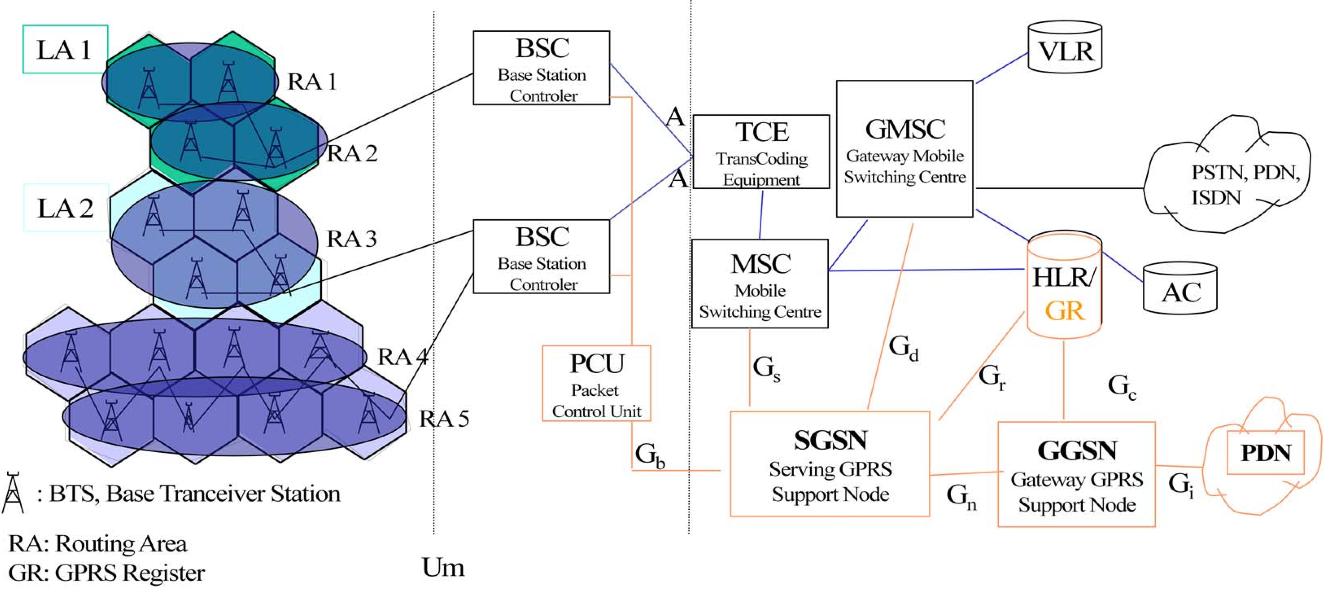
\includegraphics[width = \linewidth]{./Pics/GPRS.png} \\
Diese Grafik zeigt sehr gut, dass das GPRS kein neues Netz ist sondern eine Erweiterung von GSM. Orange eingefärbt sieht man die neuen Element. Man hat nun neben dem Verbindungsorientierten GSM Netz noch ein Paketorierntiertes GPRS Datennetz. Dieses Netz wird ausschliesslich zur Datenübertragung verwendet und kann wegen einer sehr hohen latenzzeit (bis 500ms) auch nicht für VOIP verwendet werden.

\subsubsection{Protocol stack}
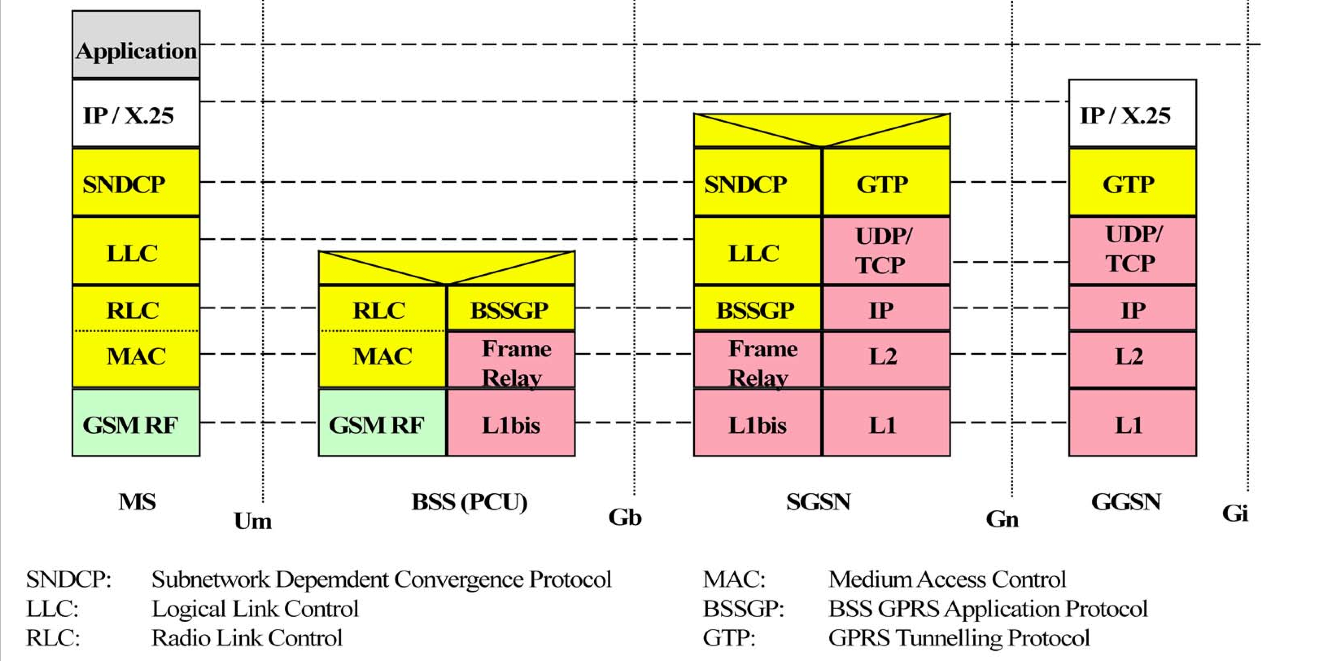
\includegraphics[width = \linewidth]{./Pics/GPRS2.png}

\begin{tabular}{|l|l|l|l|}
\hline
IP & Internet Protocol & X.25 & vorläufer von IP \\
SNDCP & Subnetwork Dependent Convergence Protocol & LLC & Logical Link Control \\
RLC  & Radio Link Control  & MAC & Medium Access Control \\
GSM RF &  Global System for Mobile Communications Radio Frequencies & BSSGP & Base Station System GPRS Protocol \\
GTP & GPRS Tunnelling Protocol & UDP & User Datagram Protocol \\
TCP & Transmission Control Protocol & & \\ 
\hline
\end{tabular}
\subsubsection{GTP}
Das GPRS Tunnelling Protocol baut IP-basierte Verbindungen durch den Backbone auf. Datenpakete werden eingepackt \& unter Benutzung des GTP getunnelt. GTP nutzt unterhalb TCP oder UDP  abhängig von der Nutzeranforderung. Das ganze GPRS Netzwerk basiert auf einem IP Hop, was das Routing im Backbone bei Mobilität vereinfacht.

\subsubsection{SNDCP - Sub Network Dependent Convergence Protocol}
\begin{itemize}
\item Konvergenz von verschiedenen Protokollen zu einem Data-Link-Protokoll (unterstütz durch das LLC)
\item Multiplext mehrere Verbindungen auf einen Link
\item Header Compression
\item Data Compression
\item Fragmentierung langer Datenpakete
\end{itemize}

\subsubsection{LLC - Logical Link Control Protocol}

\begin{itemize}
\item Etabliert eine Verbindung zwischen Mobilstation \& SGSN
\item Es kann im bestätigten oder nicht bestätigtem Modus arbeiten
\item Regelung der Datenübertragungswiederholung im bestätigten Modus
\item Unterstützung von point-to-multipoint Adressierung
\end{itemize}

\subsubsection{RLC - Radio Link Control Protocol}

\begin{itemize}
\item Arbeitet im Bestätigungs-Modus
\item Benutzt den sliding window Mechanismus für die Flusskontrolle
\item Benutzt den Packet Data Treffic Channel
\item Die Bündelung von bis zu 8 PDTCH pro User ist möglich
\item 1 PDTCH hat eine Datenrate von max. 21.4 kbit/s. Daraus ergibt sich die maximale Datenrate von 8 gebündelten PDTCH $\cdot$ 21.4 kbit/s = 171.2 kbit/s
\end{itemize}

\subsubsection{Logische Kanäle des GPRS}
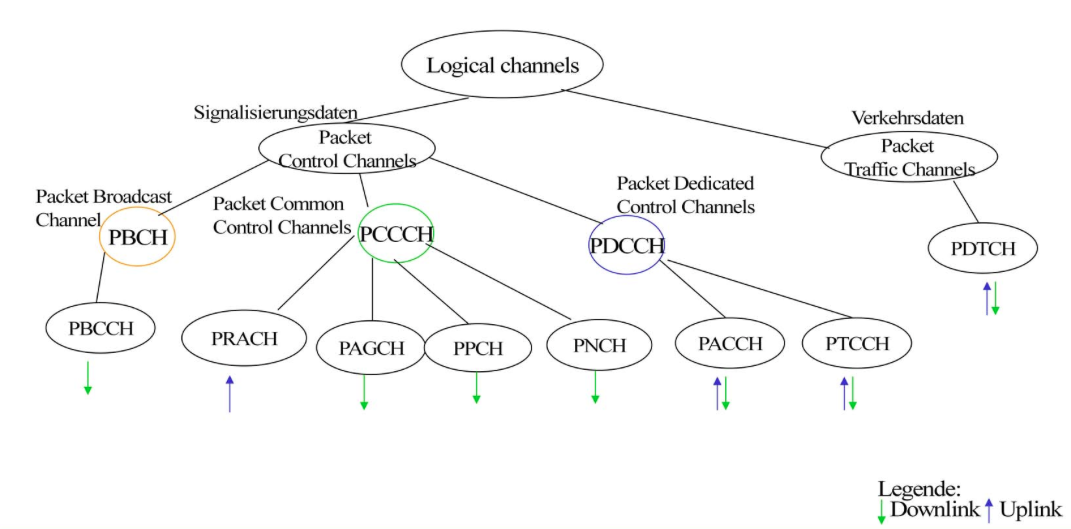
\includegraphics[width = 0.6 \linewidth]{./Pics/GPRSKanaele}

\begin{tabular}{p{0.15 \linewidth} p{0.15 \linewidth} p{0.3 \linewidth} p{0.3 \linewidth}}
\toprule
Logischer Kanal & Richtung & BTS & MS \\
\midrule
PACCH - Packet Associated Control Channel & Downlink and Uplink point to point & Sendet signalisierungsrelevante Information an die MS, z.B. Power Control, acknowledgements. Teilt sich Ressourcen mit dem PDTCH. & Empfängt Signalisierungsdaten und sendet Messreports.\\
\midrule
PAGCH - Packet Access Grant Channel & Downlink point to point & Wird benutzt in der Datenübertragungsaufbauphase zur Ressourcenzuweisung und TA Information (uplink). & Erhält die Ressourcenzuteilung ("timeslots") für den (meist uplink) Datenverkehr zu TA. \\
\midrule
PBCCH - Packet Broadcast Control Channel & Downlink point to Multipoint & Sendet allgemeine Netz/Systeminformation. Ist kein PBCCH alloziert , kann der BCCH verwendet werden. & Hört die Systeminfo ab. Ist PBCCH nicht implementiert, hört die MS den BCCH ab \\
\midrule
PDTCH - Packet Data Traffic Channel & Entweder Uplink oder Downlink Point to point/multipoint nur im DL & Daten werden übermittelt & Daten werden von MS empfangen oder gesendet. \\
\midrule
PNCH - Packet Notification Channel & Downlink point to Multipoint-Multicast & Notification an eine Gruppe von Mobilstationen, wenn multicast traffic ansteht. Wird zur Zuweisung der benötigten Ressourcen ("timeslot") verwendet & Zuweisung der timeslots\\
\midrule
PPCH - Packet Paging Channel & Downlink point to point & Wird hauptsächlich benutzt, um einen downlink Paketdatentransfer einzurichten. Der PPCH kann für Paketservice oder Circuit Switched Services verwendet werden. & Erhält die Ressourcenzuteilung ("timeslots") für den downlink Datenverkehr. \\
\midrule
PRACH - Packet Random Access Channel & Uplink point to point & Ermittelt die Timing Advance info & Benutzt die MS, um einen uplink Transfer zu etablieren \\
\midrule
PTCCH - Packet Timing Advance Control Channel & Entweder uplink oder downlink point to point & Ermittelt TA durch erhalt von Access Burst (erhalt durch UL) Sendet TA an eine Stadtion. & Sendet Access Burst zur BS. Wendet TA an. \\
\bottomrule
\end{tabular}

\subsubsection{Session Setup}

\begin{minipage}{0.5 \linewidth}
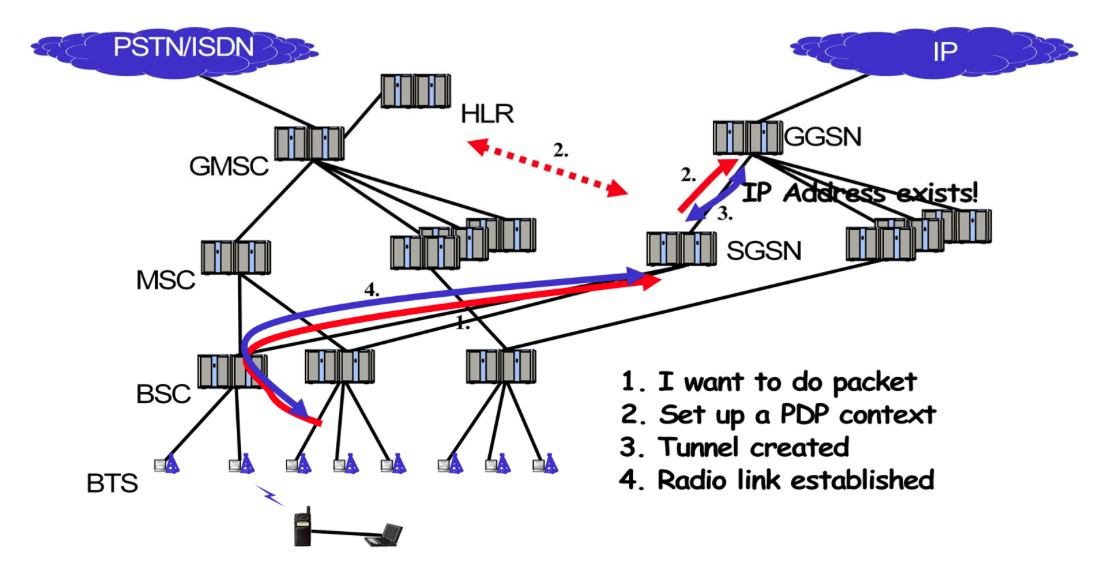
\includegraphics[width = \linewidth]{./Pics/SessionSetup} \\

\includegraphics[width = \linewidth]{./Pics/Packetdownlink} \\

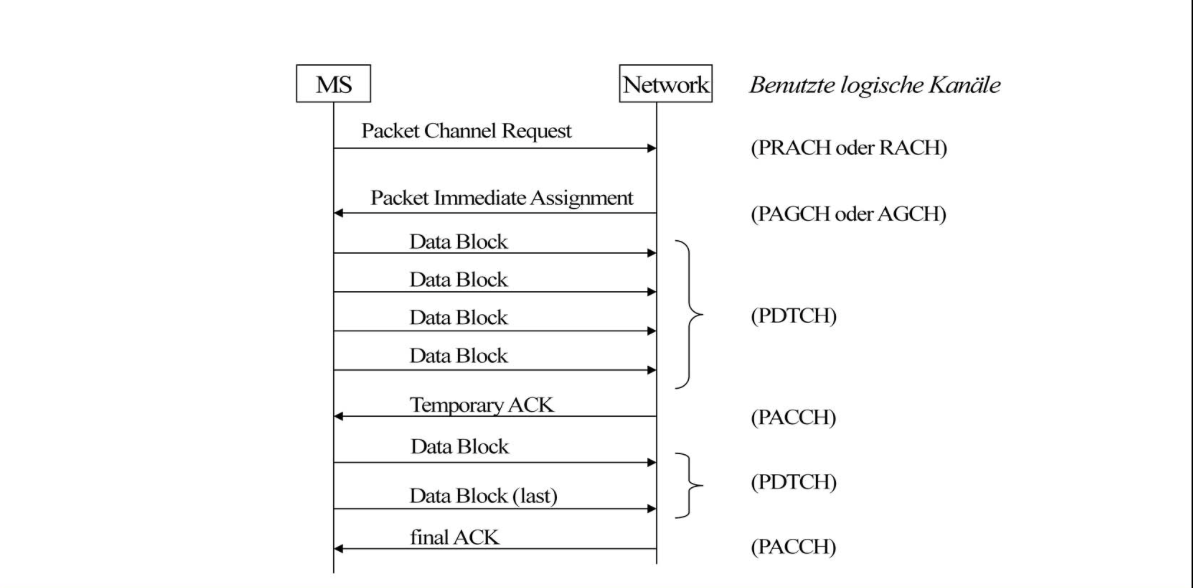
\includegraphics[width = \linewidth]{./Pics/MSDatenverkehr} \\

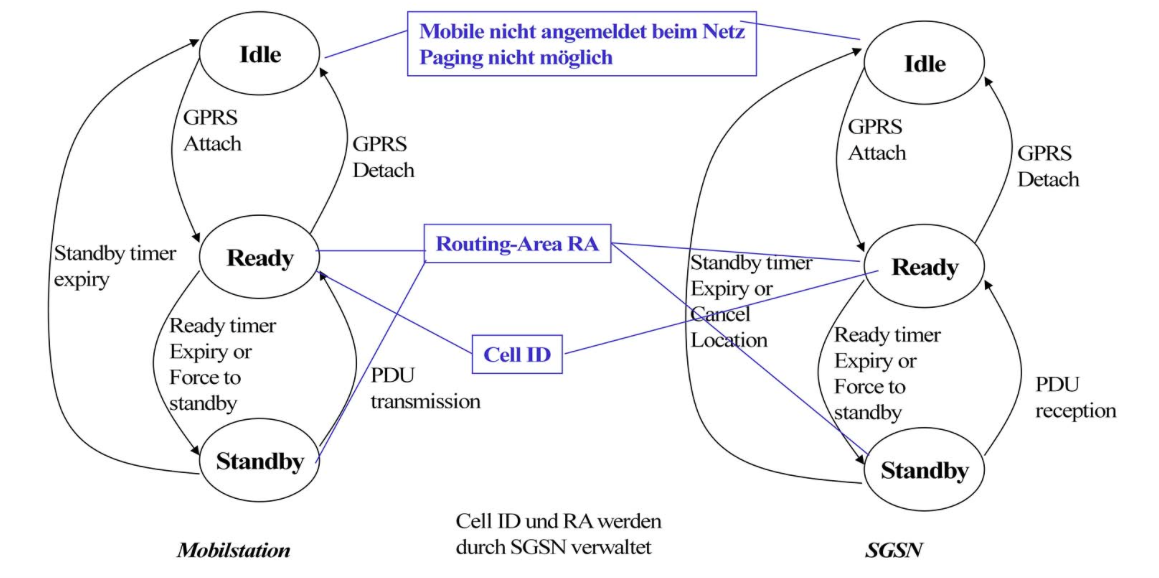
\includegraphics[width = \linewidth]{./Pics/GPRSZustandsdarstellung} \\
\end{minipage}
\begin{minipage}{0.5 \linewidth}
\begin{itemize}
\item UE meldet sich bei SGSN an
\item SGSN speichert Daten zur Mobilität und Sicherheit der MS
\item zum senden von Daten, muss UE PDP context aktivieren in SGSN  und GGSN
\item PDP context - Packet Data Protocol Context
\begin{itemize}
\item Beinhaltet alle notwenigen Informationen zum Datentranfer zwischen MS und GGSN über die PS domain
\begin{itemize}
\item MS IP adresse
\item Name des gewünschten Service/Netzwerks
\item mögliche Beschreibung des gesendeten Traffic
\item QoS Profil 
\end{itemize}
\item QoS Profil in PDP context gehört nur zum Radio link nicht zum Core Network. 
\item Im CN wird best effort IP verwendet
\item PDP context kann während einer Session nur vom SGSN verändert werden
\end{itemize}
\end{itemize}

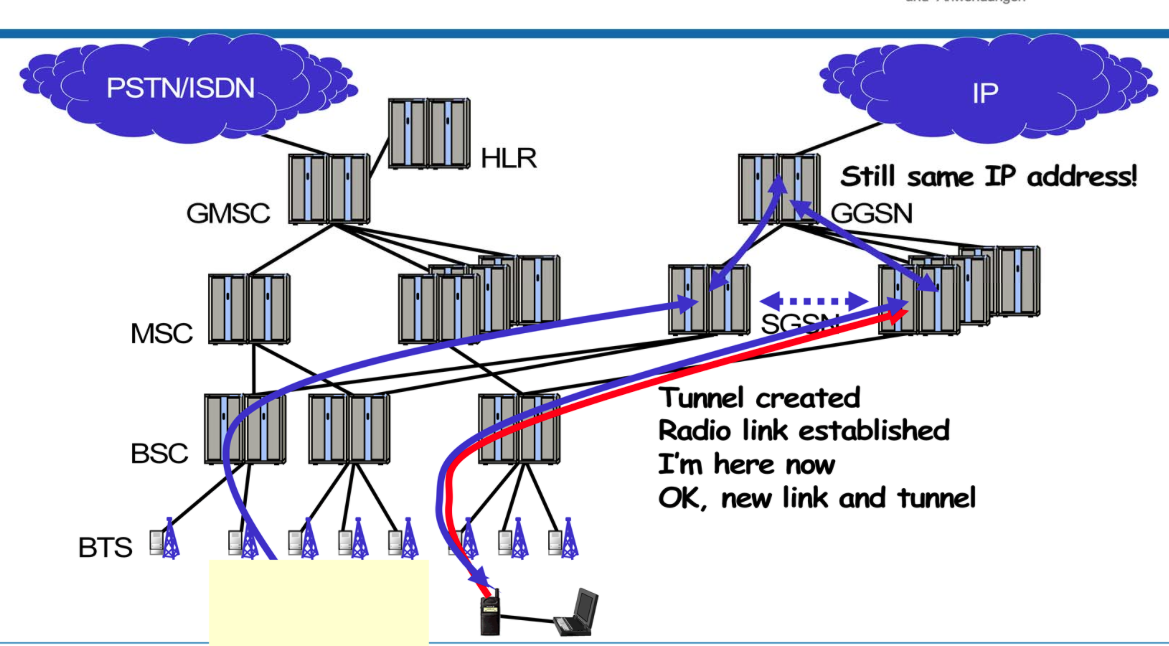
\includegraphics[width = \linewidth]{./Pics/changingSGSN} \\

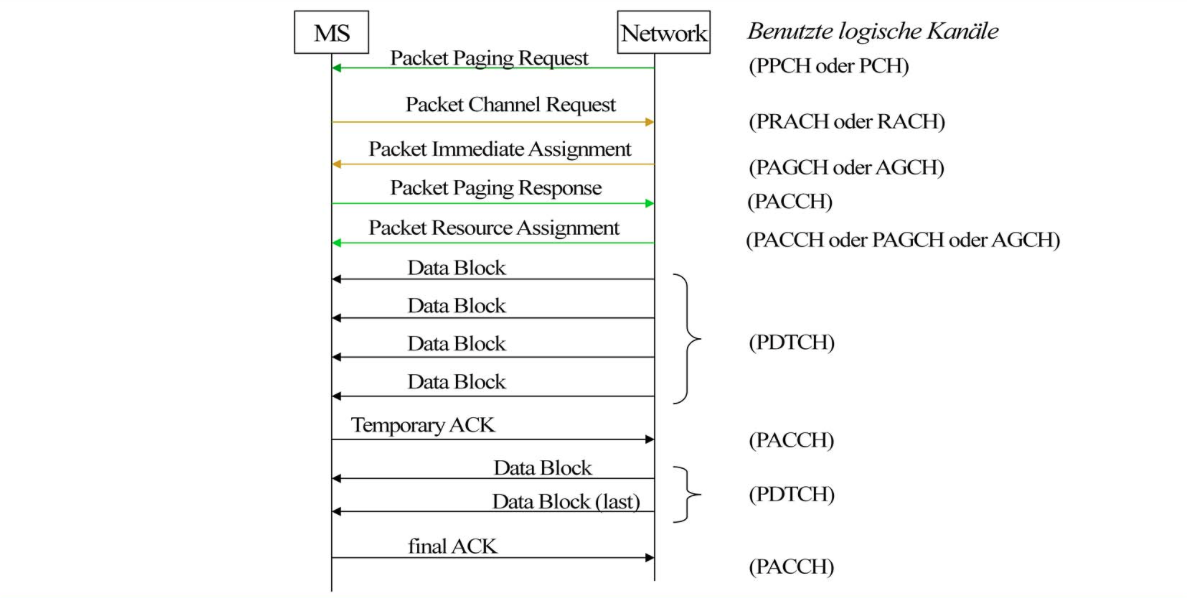
\includegraphics[width = \linewidth]{./Pics/MSDatenverkehr2} \\

\begin{itemize}
\item Im Ready Zustand
\begin{itemize}
\item der exakte Aufenthaltsort der MS ist bekannt (ID der Zelle)
\item ankommende Daten für die MS können sofort an die PCU weitergeleitet werden, wo dann die Ressourcen (Timeslots) der MS zugeteilt werden
\item Es ist kein Paging nötig
\end{itemize}
\item Im Standby Modus muss die MS gepaged werden.
\end{itemize}
\end{minipage}

\begin{minipage}{0.5 \linewidth}
\includegraphics[width = \linewidth]{./Pics/interSGSN} \\
\includegraphics[width = \linewidth]{./Pics/interSGSN2} \\
\large{\textbf{GPRS leistet:}}
\begin{itemize}
\item Flächendeckender Dienst
\item Sicher, da basierend auf dem GSM Standard
\item Übliche (realistische) Übertragungsrate ca. 50 kbit/s
\item Bis vss. 2007 die  wichtigste Technologie für mobilen Datendienst
\item Wachstum in GPRS bis zu 30\% bis 2007
\item Auswahl an preiswerten, einfachen, ausgereiften und sicheren Diensten und Endgeräten
\item Genügend Bandbreite für die meisten bisher genutzten Anwendungen (veraltet)
\item Sichere Investition für die kommenden 3 Jahr (veraltet)
\item kann auch in Randgebieten genutzt werden
\item internationales roaming möglich
\end{itemize}
\end{minipage}
\begin{minipage}{0.5 \linewidth}
\begin{enumerate}
\item Die MS detektiert eine neue Rountig Area (RA) und sendet einen RA Update Request (inklusive der alten P SRES) an die neue SGSN
\item Die neue SGSN fordert die alte SGSN auf, die Subscriberdaten (MM (Mobility Management) und PDP (Packet Data Protocol, z.B. IP oder X.25) context), zu übergeben:
\begin{itemize}
\item die neue SGSN-Adresse wird gespeichert, um später die Datenpackete weiterzuleiten.
\end{itemize}
\item Optional kann eine neue Sicherheitsüberprüfung durch die SGSN durchgeführt werden.
\item Context Request ist erfolgreich abgeschlossen und die neue SGSN kann die Datenpackete der alten SGSN empfangen
\item Die alte SGSN beginnt die gepufferten PDU's weiterzuleiten
\item Die SGSN sendet die neuen Lokalisationsdaten und PDP-Context an die GGSN. Die die Aktion bestätig
\item Der HLR/RA-Eintrag der MS wird aktualisiert
\item Die alten Einträge bzgl. der MS werden im alten SGSN gelöscht.
\item Die Subscriber-Daten werden dem neuen SGSN zur Aktualisierung im RA übertragen und die neuen SGSN bestätigt die Aktion
\item Das HLR bestätigt das Locationupdate
\item Sofern eine Assoziation zwischen der alten SGSN und dem MSC/VLR besteht und mit dem Rountig Area Update Request kein VLR Location update verbunden war, wird ein LA-update durchgeführt
\item Die SGSN validiert die neue RA der MS. Ist der Eintrag in Ordnung, erhält die MS ein Rountig Area Update Accept mit neuer P-TMSI und weitern Parametern
\item Die MS bestätigt den Empfang der neuen P-TMSI mit einem Rountg Area Update Complete
\end{enumerate}
\end{minipage}